\documentclass[12pt]{article}
\usepackage{amsmath}
\usepackage[margin = 1in]{geometry}
\usepackage{graphicx}
\usepackage{booktabs}
\usepackage{hyperref}
\usepackage{cleveref}
\hypersetup{colorlinks = true, linkcolor = blue, citecolor=blue, urlcolor = blue}
\usepackage{natbib}
\usepackage{natbib}
\usepackage{float}
\usepackage{pdfpages}




\title{Selecting Team Members of The Female United States Artistic Gymnastics Team at The 2024 Paris Olympics 
Based on Performance and Stability To Maximize Success}
\author{Kathleen Houlihan\\
  Department of Statistics\\
  University of Connecticut
}


\begin{document}
\maketitle

\begin{abstract}
    
  With the whole world anticipating the success of the United States women's artistic gymnastics team, 
  it is crucial that the team of five women that are selected to represent the United States 
  are the athletes best suited to optimize success and maximize the expected medal count in Paris 2024. As there 
  are no preexisting statistical papers that methodize the selection of athletes for Olympic Gymnastic teams, 
  this paper aims to answer the question of what metric should be used to judge the Olympic candidacy of USA 
  gymnasts and to outline a statistical method that can be used presently and in the future to select the ``best'' 
  gymnasts to comprise the United States women's Olympic team in order to maximize success. Using an analytical 
  method dependent on mean and standard deviation derived parameters, this paper outlines a procedure for identifying 
  the group of five athletes who will enable the Team USA Olympic Women’s Artistic Gymnastics team to optimize 
  success through numerically evaluating each USA athlete based on both their performance and stability in order to 
  more accurately identify the ``best'' team candidates. Through application of this analytical method to present 
  USA female artistic gymnasts, Simone Biles, Shilese Jones, Konnor McClain, Kaliya Lincoln, and Jade Carey can be 
  identified as the the group of five athletes who will enable the Team USA Olympic Women’s Artistic Gymnastics 
  teams to optimize success at the 2024 Paris Summer Olympics.

\end{abstract}

\section{Introduction}
\label{sec:intro}

For decades, gymnastics has been the most watched sport in the Summer Olympics and the United 
States has been known for bringing gold medal-winning gymnasts to compete. In the 2020 
Summer Olympics games in Tokyo, the United States women's artistic gymnastics team was the only team to take 
home a medal in all six categories. Hence, the likelihood of the USA Olympic Women’s Artistic Gymnastics 
team bringing female athletes that will medal in the 2024 Paris Olympics is very probable. 
However, in the 2020 Summer Olympic games, the United States 
male artistic gymnastics team did not medal at all. As the female USA team historically earns more medals than 
the male team, the focus of this paper is aimed at identifying a method that best isolates strong female gymnasts 
that would be prime candidates for the 2024 and future Olympics. Noting that Olympic ``success'' can be interpreted in a number 
of ways, the methods of this 
paper are designed to maximize the overall medal count by maximizing the USA team's opportunities to medal in each 
category while also placing greatest importance on the team all-around medal. 


Currently there is no literature available relevant to predicting gymnastics outcomes at the 2024 
Paris Summer Olympics or at recent olympics. However, there is literature that relates to various aspects of 
the data that will be used to form my predictions. For example, the article by \citet{ScienceOfGymnastics2021} aims to determine the 
impact of individual apparatus difficulty and execution scores on overall score. 
 Additionally, the article by \citet{JonasRohleder2023} 
can also play a similar role in predicting overall 
score. Notably, this paper found that recent Olympic rule changes resulted in significantly enhanced performance 
differentiation with the execution score being the main predictor of the final score. 
Furthermore, in the article by \citet{ApparatusDifficulty2010}, the authors use regression, cluster, and ANOVA analysis to 
analyze how difficulty scores predict overall score differently across different apparatuses. However, in this 
article the authors found that while difficulty scores may have predictive tendencies for some apparatuses, 
the strength of the prediction varied drastically from apparatus to apparatus, with there being little to no 
predictive ability for some apparatuses. Ultimately, the available literature on predicting 
gymnastic success seems generally limited to how difficulty and execution scores predict overall score.


As existing literature fails to suggest how data from major domestic and international gymnastics competitions 
from the seasons leading up to the Summer Olympics can be used to identify the ``best'' Olympic team candidates, 
the analytical method presented in this paper aims to outline a procedure that takes into account data from recent 
gymnastics competitions and Olympic competition structure in order to identify the group of five athletes who will 
enable the Team USA Olympic Women’s Artistic Gymnastics team to optimize success in Paris 2024. 

The rest of this paper is organized as follows. First, I will evaluate the data that is available in order to complete 
this project in Section~\ref{sec:data}. Then, I will discuss my 
analytical methods to determine the athletes that should be sent to the Olympics from the United States 
in Section~\ref{sec:meth}. Later, I will present the results of my 
methods in Section~\ref{sec:res}. Next, I will discuss the meaning of my results, some challenges, 
and some limitations of this project in Section~\ref{sec:dis}. Finally, in  Appendix~\ref{appendix:men}, the designed statistical 
method is applied to the male team, which is anticipated to earn fewer medals than the female team, if any.


\section{Data}
\label{sec:data}

To predict which of the United States athletes are most likely to medal on the various apparatuses, 
I will be using the cleaned data that is provided by the UConn Sports Analytics Symposium data challenge 
that includes data from major domestic and international gymnastic competitions from 2022 and 2023. 
I have opted against using the older data from 2017 to 2021 as time, injuries, 
and other factors can have a large impact on the success of a gymnast, so the greatest predictor
of the Olympic outcomes in 2024 will be the most recent data.


For the purposes of this research design, when determining the most ideal female Olympic candidates, 
only data on female United States gymnasts is analyzed, presuming that the United States 
female gymnasts have a strong chance at earning medals in any category, based on the results of the 2020 Summer Olympics. 
However, several data processing steps are required to correct several inconsistencies in the data source prior to 
analytical computations being performed:

\begin{enumerate}
\item Remove any scores of zero for the purposes of knowing the true mean scores of each athlete on each 
apparatus for each successful attempt based on the assumption that these may 
be indicative of missing scores and that instances of these scores are rare.
\item Merge ``VT,'' ``VT1,'' and ``VT2'' to all be reported as ``VT'' to avoid having 
multiple statistics for one athlete on the same apparatus.
\item Convert all last names to lower case for consistency purposes.
\end{enumerate}


\section{Methods}
\label{sec:meth}

For women, the data challenge presents the task of determining 
which five athletes stand the greatest chance of winning the gold medal for the women's individual all-around,
team all-around, Balance Beam, Floor Exercise, Uneven Bars, and Vault. 

In order to reduce the list of USA gymnasts to just five athletes, the proposed method in 
this paper utilizes a parameter value of the score standard deviation multiplied by some alpha value subtracted 
from the mean score for each apparatus, or $\mu - \alpha \sigma$. This parameter value serves to rank athletes based 
on having both a high mean score for a particular event and low standard deviation. 
This alpha value is decided by examining the plots of the mean versus the standard deviation of the ten athletes 
with the highest mean scores on each apparatus. The default alpha value is 1, and ideally this produces a parameter 
value where the athletes with the highest mean scores and lowest standard deviations have the highest parameter values. 
However, in cases where the rank produced by the parameter value selects athletes with comparatively low mean scores and 
low standard deviations prior to athletes with significantly higher mean scores and slightly high standard deviations, 
this alpha value should be reduced until the rank of the athletes coordinates with the order that seems visually most 
logical based on the plots. While the parameters are to an extent subjective, in the final analysis the exact rank that 
is determined by the parameter is not terribly signifiant as the parameter values are used to determine the top five 
athletes for each apparatus and typically play the largest role in determining which athletes are included at the margin. 
Ultimately, if an athlete is bordering being 4th, 5th, 6th, or 7th best for a particular apparatus in the United States 
and the athlete is not superior on another apparatus, it is highly unlikely that they would be selected for the Olympic 
team at all. For the purposes of this research, it is reasonable to ignore any athletes who have only competed once 
on a particular apparatus and do not have a parameter value as they would 
likely not be selected to compete on that apparatus at the Olympics.

In order to select the appropriate athletes, I first processed the data as described in Section~\ref{sec:data} 
and then adhered to the following procedure:

\begin{enumerate}
  \item Determine the best individual apparatus candidates.
  \begin{enumerate}
    \item Calculate and examine the mean and standard deviations of each American female athlete's score 
    on each apparatus.
    \item Calculate the number of observations for each athlete on each apparatus.
    \item Plot the mean versus the standard deviation of the ten athletes with the highest mean scores on each 
    apparatus.
    \begin{enumerate}
      \item Use these plots as a visual to represent the possible scores that could be achieved in each apparatus 
     component of the Olympics.
     \item Using the plots, create a parameter for each apparatus that uses both mean score and standard 
     deviation to identify which athletes are best suited to be considered to compete on behalf of the United 
     States on each apparatus.
     \begin{enumerate}
       \item Select the five athletes with the highest parameter value for each apparatus to identify the ``best'' 
        five athletes that compete on each apparatus based on both their success, a high mean score, and their 
        inconsistency, their standard deviation.
     \end{enumerate}
     \item Identify the athletes with the two largest parameter values as the ``best'' on each apparatus.
    \end{enumerate}
  \end{enumerate}
  \item Determine the best individual all-around candidates.
  \begin{enumerate}
   \item Produce a list of ``target athletes'' for future computations that contains all athletes that were identified 
   as being in the top five for any apparatus in the last step.
   \begin{enumerate}
     \item Remove any athletes from the ``target athletes'' list that have not competed on all apparatuses.
   \end{enumerate}
   \item Calculate the sum of each ``target athlete's'' mean score for each apparatus and the sum of each athlete's standard 
   deviation for each apparatus.
    \item Plot the mean score sum versus the standard deviation sum for each ``target athlete.''
   \begin{enumerate}
     \item Use this plot as a visual to represent the possible scores that could be achieved in the individual all-around 
     component of the Olympics.
   \end{enumerate}
  \end{enumerate}

\item Determine the best team all-around candidates.
  \begin{enumerate}
   \item Calculate the summed mean score and standard deviation sum of every combination of three athletes using the previously 
   calculated sum of each ``target athlete's'' mean score for each apparatus and the sum of each athlete's standard 
   deviation for each apparatus.
   \item Plot the summed mean score versus the standard deviation for the ten combinations of three athletes with the 
   highest summed mean score.
   \begin{enumerate}
     \item Use this plot as a visual to represent the possible scores that could be achieved in the all-around team finals 
    component of the Olympics.
   \end{enumerate}
   \item Calculate the summed mean score and standard deviation sum of every combination of four athletes using the previously 
   calculated sum of each ``target athlete's'' mean score for each apparatus and the sum of each athlete's standard 
   deviation for each apparatus.
   \item Plot the summed mean score versus the standard deviation for the ten combinations of four athletes with the 
   highest summed mean score.
   \begin{enumerate}
      \item Use this plot as a visual to represent the possible scores that could be achieved in the all-around team qualifying  
     round of the Olympics.
   \end{enumerate}
  \end{enumerate}
  
\item Visually examine each produced plot to build a final team of five in an effort to include in 
    the final team the best three candidates for the team all-around, the best candidate for the fourth qualifying position, 
    the best two candidates for the individual all-around, and the two athletes that are superior on each apparatus.
\end{enumerate}

    


\section{Results}
\label{sec:res}

\begin{figure}
  \centering
  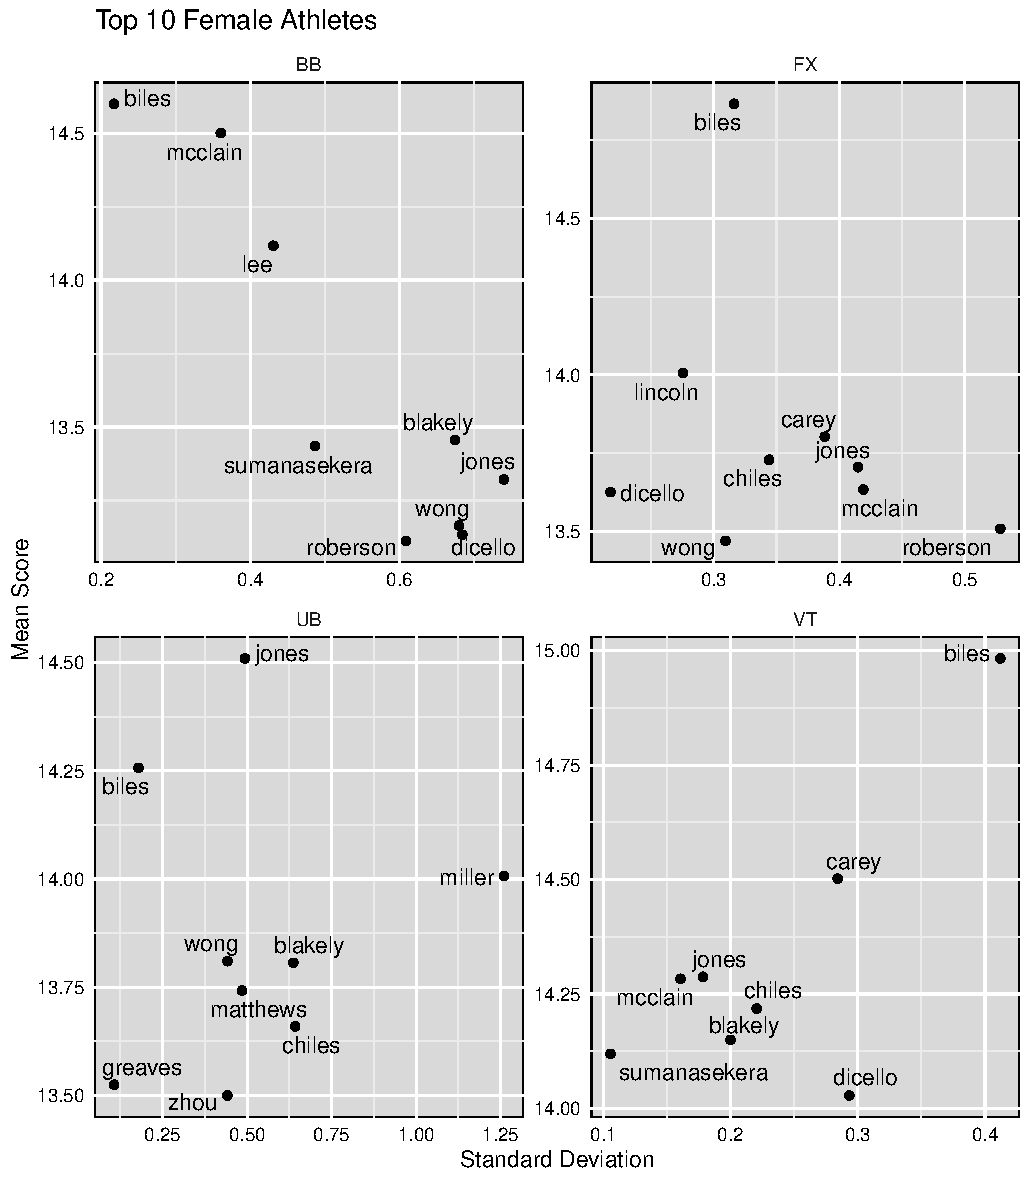
\includegraphics[scale=0.7]{FinalFemaleApparatusPlot.pdf}
  \caption{Top 10 Female Candidates for the Olympic Balance Beam, Floor Exercise, Uneven Bars, and Vault Apparatus.}
  \label{fig:FA}
\end{figure}

\begin{table}
  \caption{Top ten female candidates for each apparatus based on mean score alone and 
  their $\mu - \alpha \sigma$ parameter values.}
  \label{table:1}
\centering
\begin{tabular}[t]{llllllll}
 \toprule
  \multicolumn{2}{c}{BB} & \multicolumn{2}{c}{FX} & \multicolumn{2}{c}{UB} & \multicolumn{2}{c}{VT}\\
  \cmidrule(lr){1-2}\cmidrule(lr){3-4}\cmidrule(lr){5-6}\cmidrule(lr){7-8}
Athlete & $\mu - \sigma$ & Athlete & $\mu - \sigma$ & Athlete & $\mu - 0.5 \sigma$ & Athlete & $\mu - 0.5 \sigma$\\
\midrule
biles & 14.38 & biles & 14.55 & jones & 14.26 & biles & 14.78\\

mcclain & 14.14 & lincoln & 13.73 & biles & 14.17 & carey & 14.36\\

lee & 13.69 & carey & 13.41 & wong & 13.59 & mcclain & 14.20\\

sumanasekera & 12.95 & dicello & 13.4 & matthews & 13.50 & jones & 14.20\\

blakely & 12.78 & chiles & 13.38 & blakely & 13.49 & chiles & 14.11\\

jones & 12.58 & jones & 13.29 & greaves & 13.47 & sumanasekera & 14.07\\

roberson & 12.50 & mcclain & 13.21 & miller & 13.38 & blakely & 14.05\\

wong & 12.48 & wong & 13.16 & chiles & 13.34 & dicello & 13.88\\

dicello & 12.45 & roberson & 12.98 & zhou & 13.28 & richardson & NA\\

frazier & NA & frazier & NA & walker & NA & torry & NA\\
\bottomrule
\end{tabular}
\end{table}

Based on the plot of the top ten female athletes on the balance beam apparatus in Figure~\ref{fig:FA} I selected the parameter of 
the score standard deviation subtracted from the mean score in order to identify the best suited five 
athletes. Based on the parameter displayed in Table~\ref{table:1}, the five ``best'' female athletes on balance beam are Biles, McClain, 
Lee, Sumanasekera, and Blakely with Biles and McClain being expert for this apparatus. Similarly, the five ``best'' 
female athletes for floor exercise are Biles, Lincoln, Carey, 
Mcclain, Dicello, Chiles with Biles and Lincoln being expert for this apparatus. Based on the plot of the top ten 
female athletes on the uneven bars apparatus I selected the parameter of 
half of the score standard deviation subtracted from the mean score in order to identify the best suited five 
athletes. Based on the parameter, the five ``best'' female athletes for uneven bars are Jones, Biles, Wong, 
Matthews, and Blakely with Jones and Biles being expert for this apparatus. Similarly, the five ``best'' female 
athletes on vault are Biles, Carey, Mcclain, Jones, 
and Chiles with Biles and Carey being expert for this apparatus.

\begin{figure}
  \centering
  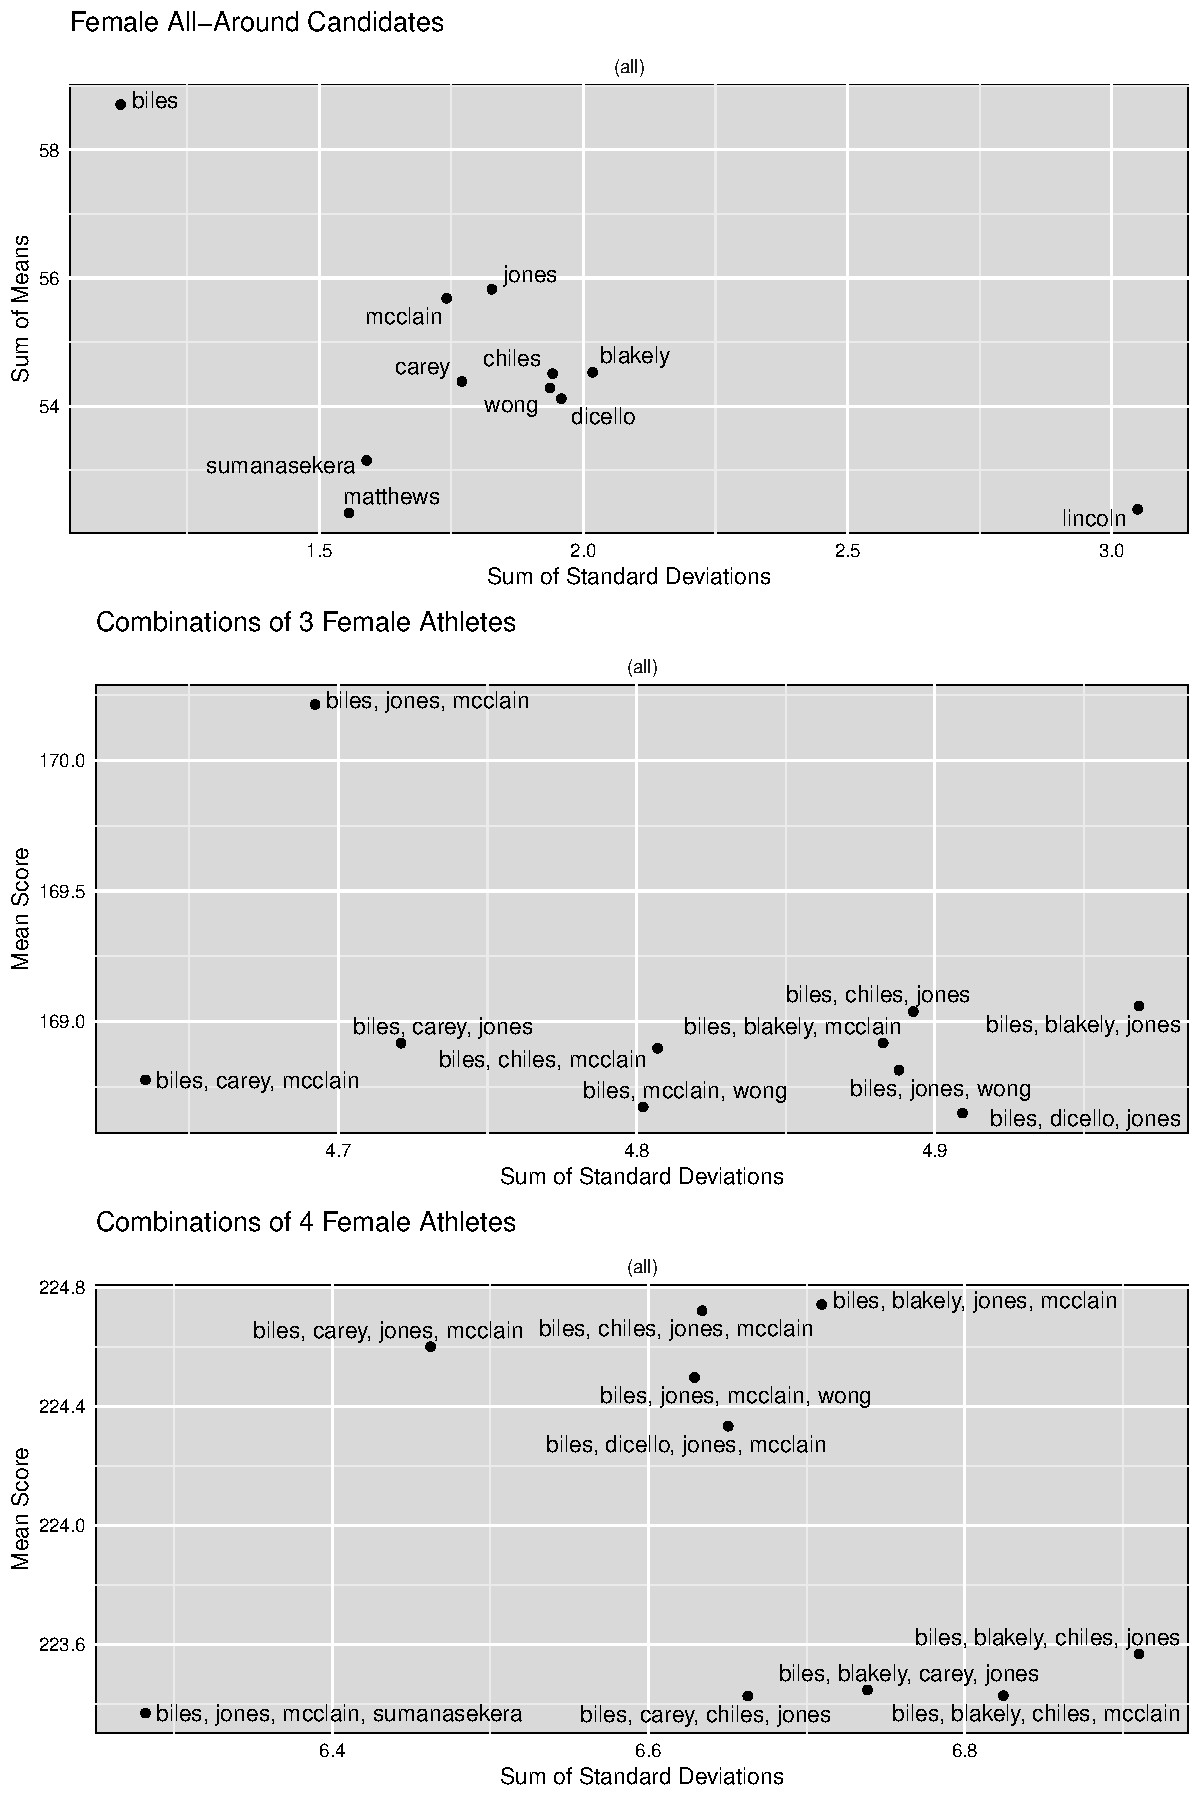
\includegraphics[scale=0.55]{FinalFemaleAllAroundPlot.pdf}
  \caption{The best candidates for the female individual all-around and team all around medals.}
  \label{fig:FAA}
\end{figure}

Based on the plots in Figure~\ref{fig:FAA}, it is very clear that Biles is strong candidate to 
compete for the individual all-around medal. Looking at the data values and plot of the combinations of three athletes, 
it is clear that Biles, Jones, and McClain are by far the best suited trio to compete for the team all-around medal. 
Looking at plot of the combinations of four athletes, it is not clear whether Chiles, Carey, or 
Blakely is best suited to be the fourth team all-around candidate as their means and standard deviations are very 
similar. However, based on the computations and plots, the superior two 
athletes on balance beam are Biles and McClain, the superior two athletes on floor exercise are Biles and Lincoln, 
the superior two athletes on uneven bars are Jones and Biles, and the superior two athletes on vault are Biles 
and Carey. Since Lincoln was not among our top candidates for an all-around medal, it would be logical to select her 
as the fifth United States Olympic team member who does not compete in the all-around qualifying round. Additionally, 
since Carey is one of the candidates being considering for the all-around qualifying round and she is one of our superior 
athletes on vault, it is reasonable to also select her to be the final member of the Olympic team. 

Hence, based on the proposed method, in order to maximize the number of medals the Unites States female team wins, 
the team should be comprised of the athletes Biles, Jones, McClain, Lincoln, and Carey.
 
\section{Discussion}
\label{sec:dis}

Using an analytical method dependent on mean and standard deviation derived parameters, this paper 
outlines a procedure for identifying the Team USA Olympic Women’s Artistic Gymnastics team that will optimize 
success at the Olympics through numerically evaluating each USA athlete based on both their accuracy and precision. 
Ultimately, Simone Biles, Shilese Jones, Konnor McClain, Kaliya Lincoln, and Jade Carey can be identified as the 
the group of five athletes who will enable the Team USA Olympic Women’s Artistic Gymnastics teams to optimize 
success at the 2024 Paris Summer Olympics based on this method.

At various steps throughout the procedure large quantities of athletes were eliminated from consideration 
based on various analytical decisions. For example, most athletes were eliminated from consideration as 
only athletes that ranked in the top ten by mean score alone for each apparatus were inspected. This was a 
reasonable elimination of data as the score values among the top ten candidates varied enough, often by over a 
full point, to justify that athletes that never ranked in the top ten for a particular apparatus are not 
competitive enough to medal at the Olympics. Furthermore, this list of athletes was also reduced by half by the 
use of a subjectively determined parameter, but this decision is also justified as only two athletes from each 
country can compete for an apparatus medal, so reducing the considered candidates to only the top five for each 
apparatus is reasonable as it would be highly unlikely for the 6th best USA candidate for a particular apparatus 
to medal at the Olympics.

Notably, this algorithm is not powerful for strong athletes with few attempts on a particular apparatus as individuals 
with only one attempt could not possess a parameter value and thus were eliminated. Additionally, this algorithm 
would not be strong for a country that is inferior at certain events as this model assumes athletes from the country 
of interest have a reasonable chance at medaling in any category. As such, this model is designed to have the strongest 
candidates competing in every category regardless of global rank in each category.

Furthermore, the design of this method does not take into account the impact of difficulty or execution scores on 
overall score. While this data could have been beneficially in selecting the most competitive or successful athletes 
to comprise the Olympic team, existing literature doubted whether difficulty and execution scores should be 
used as predictors at all.

Ultimately, while this analytical method may not take into account all of the information and that that was available, 
the method was able to identify a competitive group of athletes that represent the ``best'' athletes suited 
to medal and optimize success in each of the Olympic events.


\appendix

\section{Application of Methods To The Male USA Artistic Gymnastics Team}
\label{appendix:men}

\begin{figure}
  \centering
  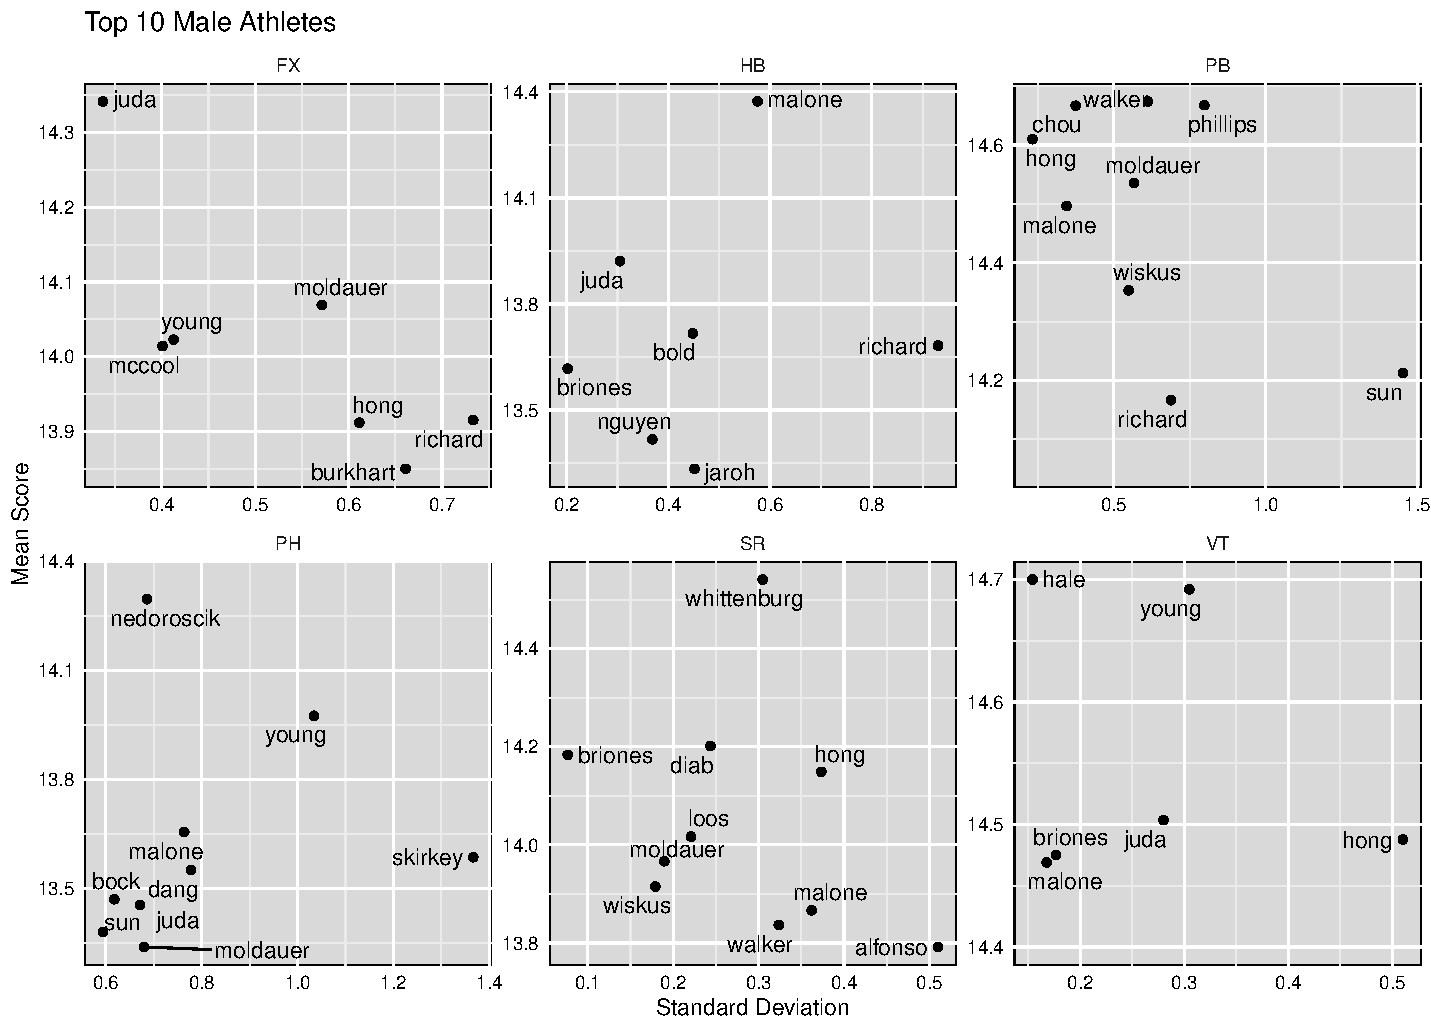
\includegraphics[scale=0.5]{FinalMaleApparatusPlot.pdf}
  \caption{Top 10 Male Candidates for the Olympic Floor Exercise, Pommel Horse, Still Rings, Vault, Parallel Bars, 
  and High Bar Apparatus.}
  \label{fig:MA}
\end{figure}

\begin{figure}
  \centering
  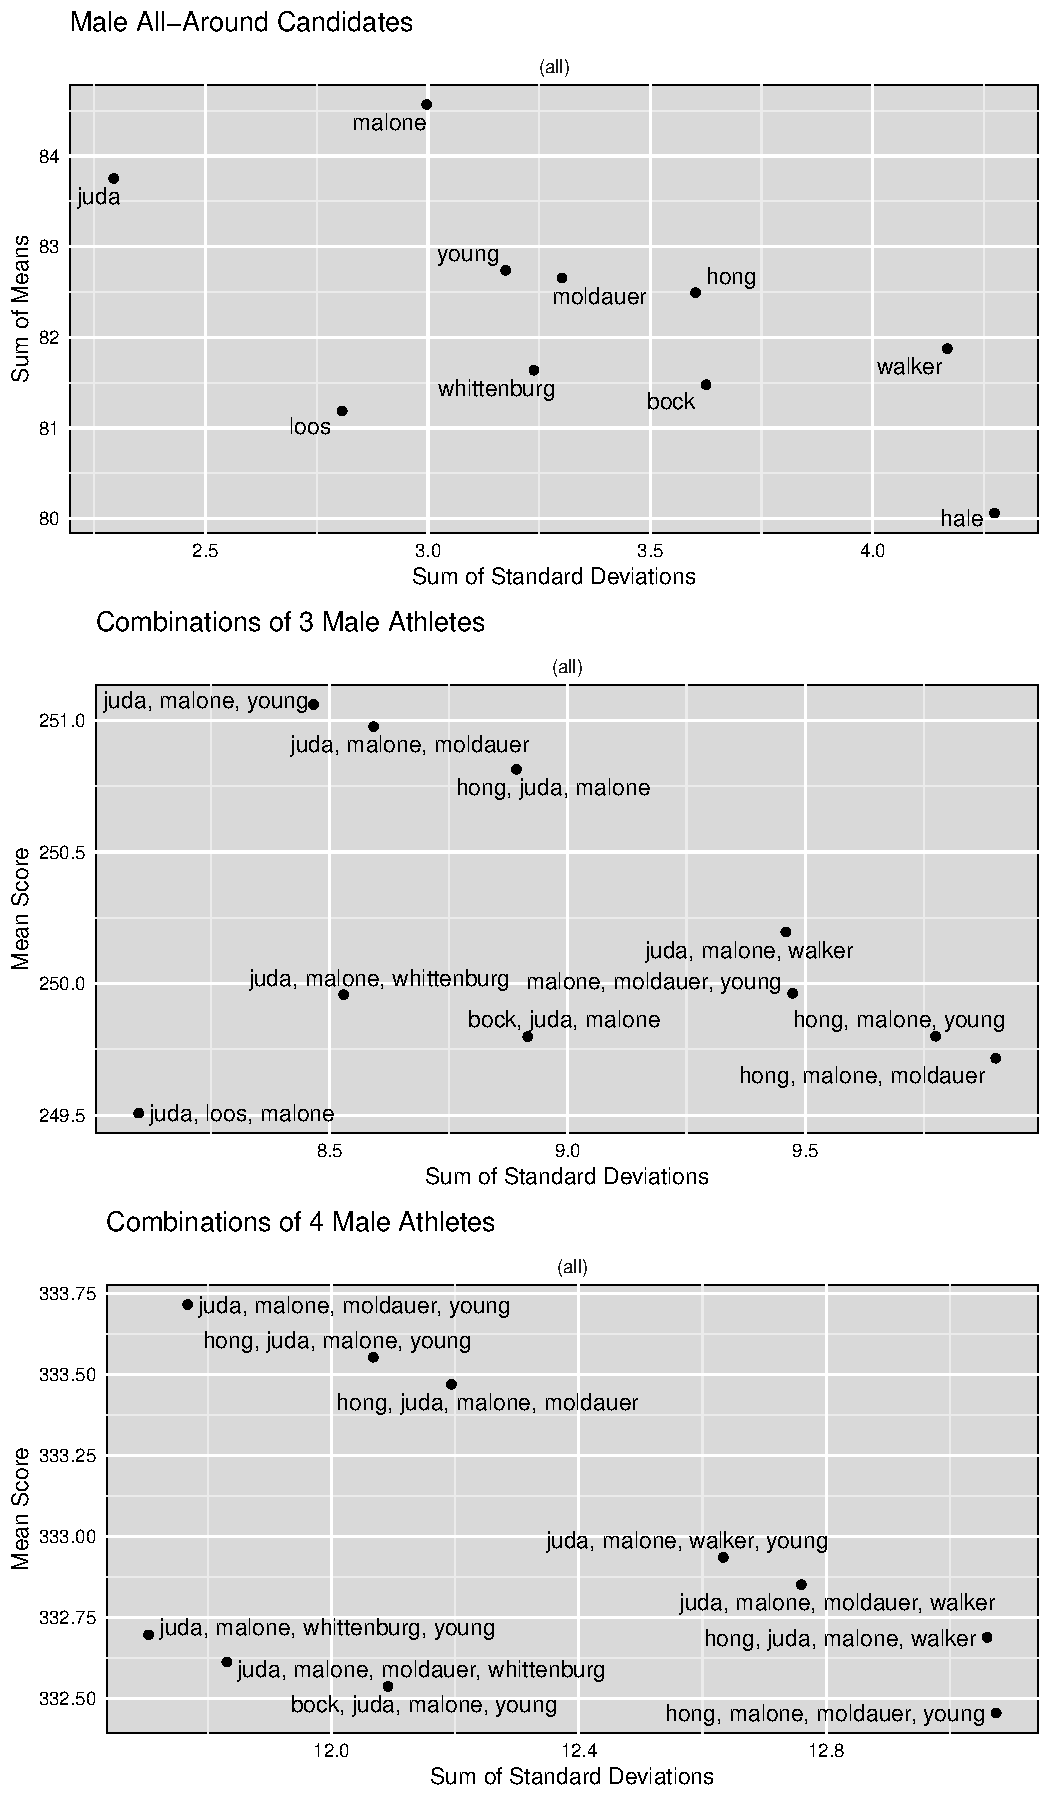
\includegraphics[scale=0.7]{FinalMaleAllAroundPlot.pdf}
  \caption{The best candidates for the male individual all-around and team all around medals.}
  \label{fig:MAA}
\end{figure}


For men, the overall statistical method I used to determine the team of five male gymnasts that should be sent 
to the 2024 Olympics was very similar, but varied when it came to determining the final fifth team member. After 
using the same method to determine the United States' best four male candidates for the team all-around qualification 
round, I calculated the mean score for every male gymnast on every apparatus in order to determine which apparatuses 
the male USA team had the greatest chance of earning medals on. From this data, there was only one additional male 
USA gymnast that ranked globally in the top ten for a particular apparatus based on mean score alone. 
Ultimately, in order to maximize the the number of medals the Unites States male team wins, the team should be comprised  
of the athletes Juda, Malone, Young, Moldauer, and Hale.

\bibliographystyle{chicago}
\bibliography{citations}

\end{document}